\subsection{template fitting of $d(K^-, n \pi^+ \pi^-)"n"$ final state}  \label{sec:tempfit}

$K^0$ tagged spectrum is seems to quasi-elastic scattering which will be rised from the $\bar{K}N$ threshold due to fermi motion.
Strangeness was teken forward in $\Sigma_{forward}$ tagged events, so these are naturally expected to 1-step raction.
$K^-$-proton reactions have been studied about various final states and widly energy region\cite{CERN_HARA_K},
ofcouse $K^-p\rightarrow K^0 n$ and $K^-p\rightarrow \pi^{\mp}\Sigma^{\pm}$ with $1GeV/c$ $K^-$ have been studied\cite{KP_MB}.
Fermi motion in deuteron also have been studied from both theoretical and experimental side.
So, we can simulate these quasi-elastic reactions.
Angular distribution of $K^-$ one nucleon reactions were simulated previous experimental data
and the other nucleon was regarded as spectator whose momentum was distributed fermi motion which was simulated previous expermental of $d(e, e'p)"n"$ reaction\cite{d_fermi_ex}.

$d(K^-, n)"\pi^{\mp}\Sigma^{\pm}"$ reaction is regarded as 2-step reaction which is no data. 
In $d(K^-, n)"\pi^{\mp}\Sigma^{\pm}"$, detected neutron acceptance was restricted for super-forward angle so simulation data was produced using neutron angle within 8degree.
Becouse momentum transfer around the $\bar{K}N$ threshold is small, the $\bar{K}N \rightarrow \pi^{\mp}\Sigma^{\pm}$ scattering is expected to S-wave.
We adopt isotropic angular distribution in $\pi^{\mp}\Sigma^{\pm}$ decay.
We adopt flat mass distribution of $\pi^{\mp}\Sigma^{\pm}$ from the $\bar{K}N$ threshold to 1.8 $GeV/c^2$ due to small phase space around the $\bar{K}N$ threshod.

We made 5 type template data using Geant4 which is Monte Carlo simulation toolkit for particle and nuclear physics\cite{geant4} as follow.
\begin{eqnarray}
& &  K^- d \rightarrow n K^0 n_{spectator} \mbox{(1-step reaction)} \label{1step:K0} \\
& &  K^- d \rightarrow \pi^- \Sigma^+ n_{spectator} \mbox{(1-step reaction)} \label{1step:pimSp} \\
& &  K^- d \rightarrow \pi^+ \Sigma^- n_{spectator} \mbox{(1-step reaction)} \label{1step:pipSm} \\
& &  K^- d \rightarrow \pi^- \Sigma^+ n_{forward} \label{2step:pimSp} \\
& &  K^- d \rightarrow \pi^+ \Sigma^- n_{forward} \label{2step:pipSm}
\end{eqnarray}
The detail of the Monte Carlo using Geant4 was described in Set\ref{sec:geant4}.

These reactions was decomposed by so-called template fitting\cite{tempfit}.
In this fitting, scaling factors are free parameters which was adjusted to reproduce the data spectrum and the criteria of goodness was adopted poisson/canonical distribution,
so the template fitting considered statistics of the data spectrum and expected spectra.

There are two type fittings for the decomposition.
One is invariant mass fitting of $\pi^+ \pi^-$ and $n \pi^{\pm}$ for $K^0$ and $\Sigma^{\pm}_{forward}$ production.
$K^0$ and $\Sigma^{\pm}_{forward}$ peaks could be reconstructed from invariant masses of $\pi^+ \pi^-$ and $n \pi^{\pm}$, respectively.
The other is  $d(K^-, n \pi^{\mp})"X"$ fitting for decomposition of the $\pi^{\mp}\Sigma^{\pm}$ modes.
The $\pi^-\Sigma^+$ mode make $d(K^-, n \pi^-)"\Sigma^+"$ peak and widly distributes in $d(K^-, n \pi^-)"X"$ spectrum. 
Opposite charge is same as.

\begin{figure}
  \begin{tabular}{ccc}
    \begin{minipage}{0.33\hsize}
      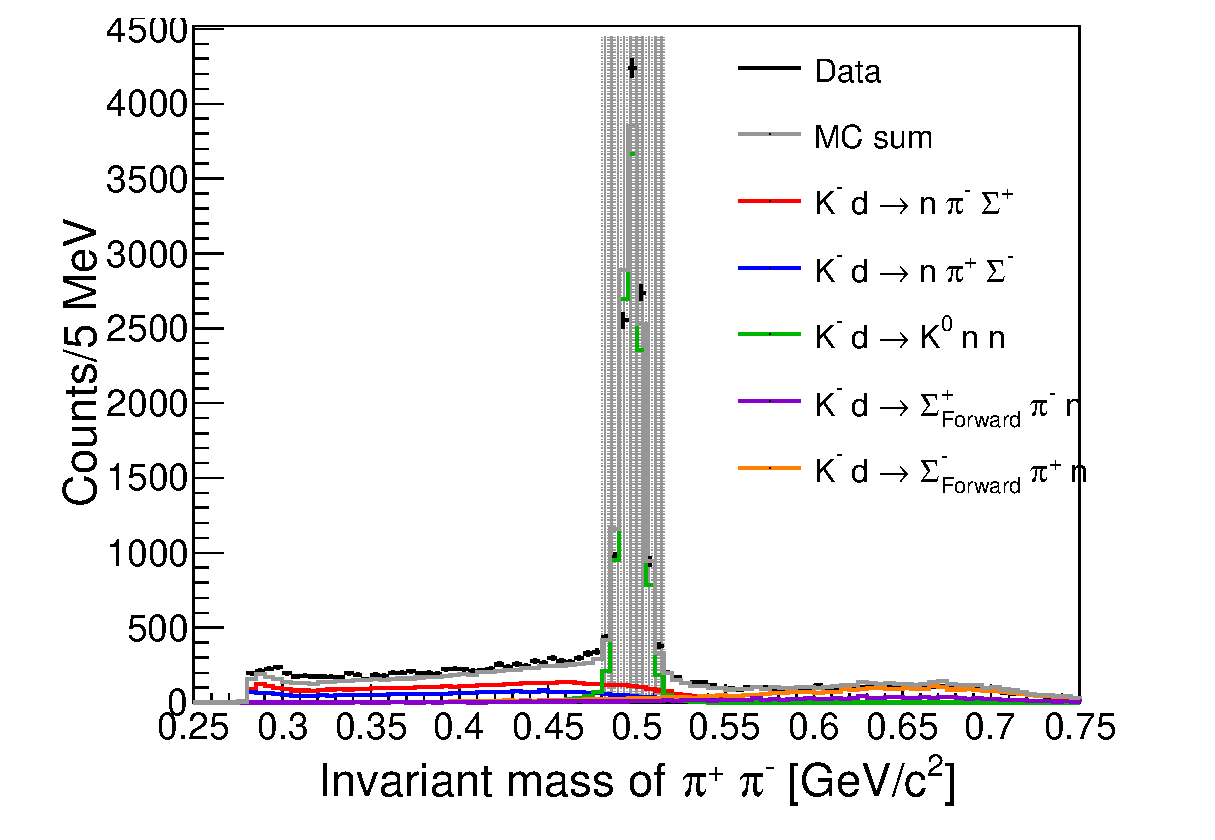
\includegraphics[width=4cm]{../pic/Run78/KN_ana_NC170_2sigma/IM_pipi.eps}
    \end{minipage}
    \begin{minipage}{0.33\hsize}
      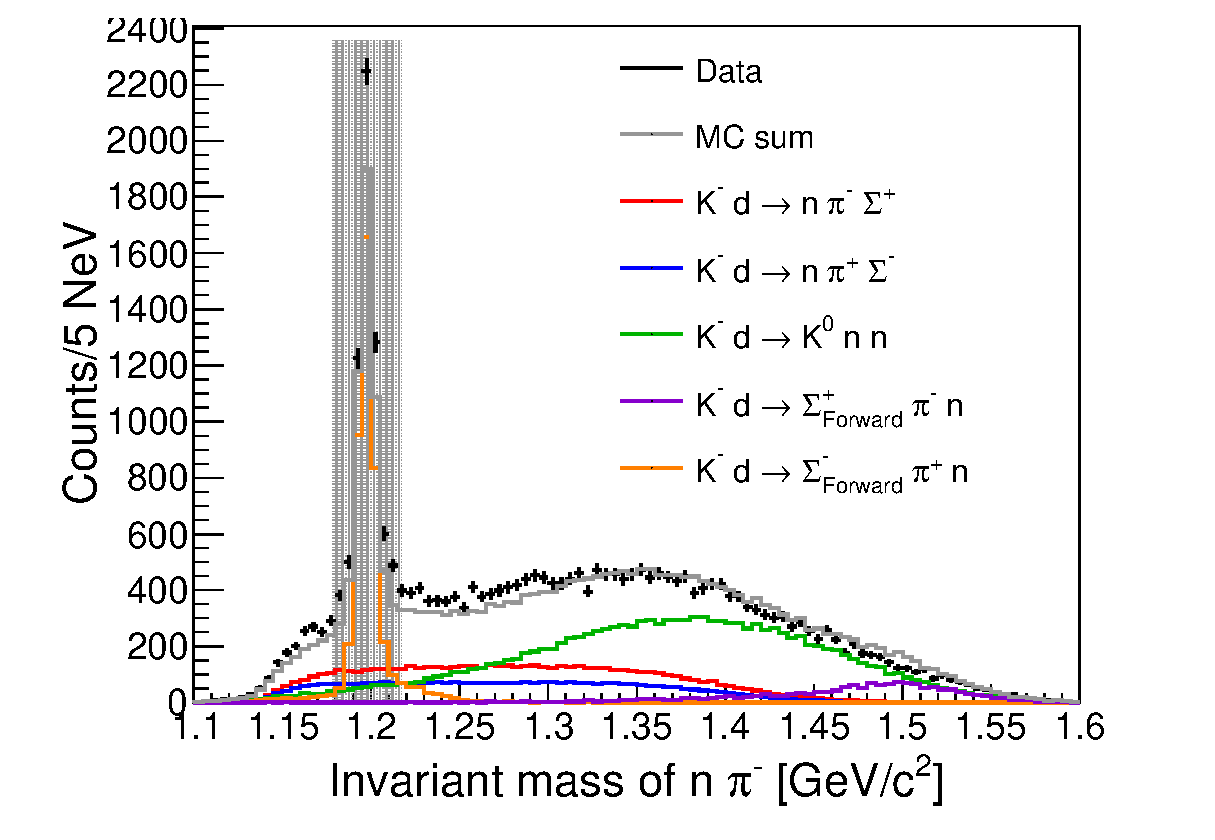
\includegraphics[width=4cm]{../pic/Run78/KN_ana_NC170_2sigma/IM_npim.eps}
    \end{minipage}
    \begin{minipage}{0.33\hsize}
      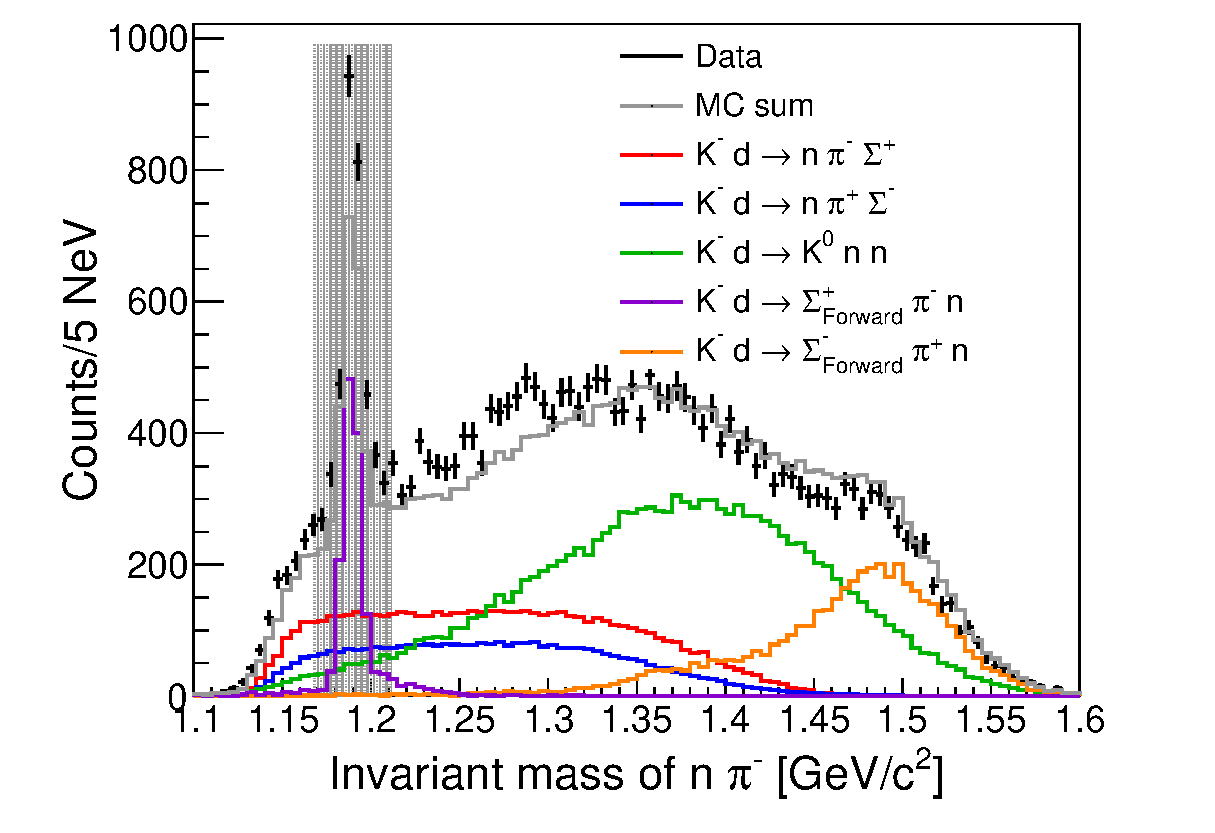
\includegraphics[width=4cm]{../pic/Run78/KN_ana_NC170_2sigma/IM_npip.eps}
    \end{minipage}
  \end{tabular}
  \caption{
    These figures shows invariant masses of $\pi^+ \pi^-$, $n \pi^-$ and $n \pi^+$ with fitting result of 5 reactions.
  }
  \label{fig:IM_fit}
\end{figure}

The reactions(\ref{1step:K0}-\ref{1step:pipSm}) can be simulated using angular distribution and fermi motion of the spectator that was well studied,
so these reactions use same template around whole events.
On the other hand, there are no data about the branching ratio of the $d(K^-, n)"\pi^{\mp}\Sigma^{\pm}"$ modes that should be depend on the $\pi^{\mp}\Sigma^{\pm}$ mass.
We should decompose each $d(K^-, n)"\pi^{\mp}\Sigma^{\pm}"$ modes each $\pi^{\mp}\Sigma^{\pm}$ mass from the data.
For the reason, the fitting of the $d(K^-, n \pi^{\mp})"\Sigma^{\pm}"$ was performed bin-by-bin of the $d(K^-, n)"X"$.
Since the purpose of this analysis is determination of the ratio of the $"\pi^{\mp}\Sigma^{\pm}$ modes,
We adopted this fitting to events rejected $K^0$ and $\Sigma^{\pm}_{forward}$.

We iteratively performed these fittings and the other parameters were fixed.
Thus, the $d(K^-, n)"\pi^{\mp}\Sigma^{\pm}"$ spectra were fixed in the invariant mass fitting.
On the other hand, spectra simulated 1-step $K^0$ and $\Sigma^{\pm}_{forward}$ reactions were fixed in the $d(K^-, n \pi^{\mp})"X"$ fitting.

We estimated each reactions' template spectra of $\pi^+ \pi^-$ and $n \pi^{\pm}$ invariant masses as Fig\ref{fig:IM_fit}.
Although the $d(K^-, n \pi^{\mp})"X"$ fitting was adopted to events rejected $K^0$ and $\Sigma^{\pm}_{forward}$ ,
contamination from these reactions was estimated from invariant mass fittings which was considered in the $d(K^-,n \pi^{\pm})"X"$ fitting. 
The $d(K^-, n \pi^{\mp})"X"$ spectra were reproduced as shown in Fig\ref{fig:KN_MM_woAll}.
The $d(K^-, n \pi^{\mp})"X"$ fitting was performed each bins of $d(K^-, n)"\pi^{\mp}\Sigma^{\pm}"$ whose likelihood was shown in same figure.
Reproduced spectra in each bin were also shown in Fig\ref{fig:KNpi_MM_fit_div}

\begin{figure}[htbp]
  \centering
  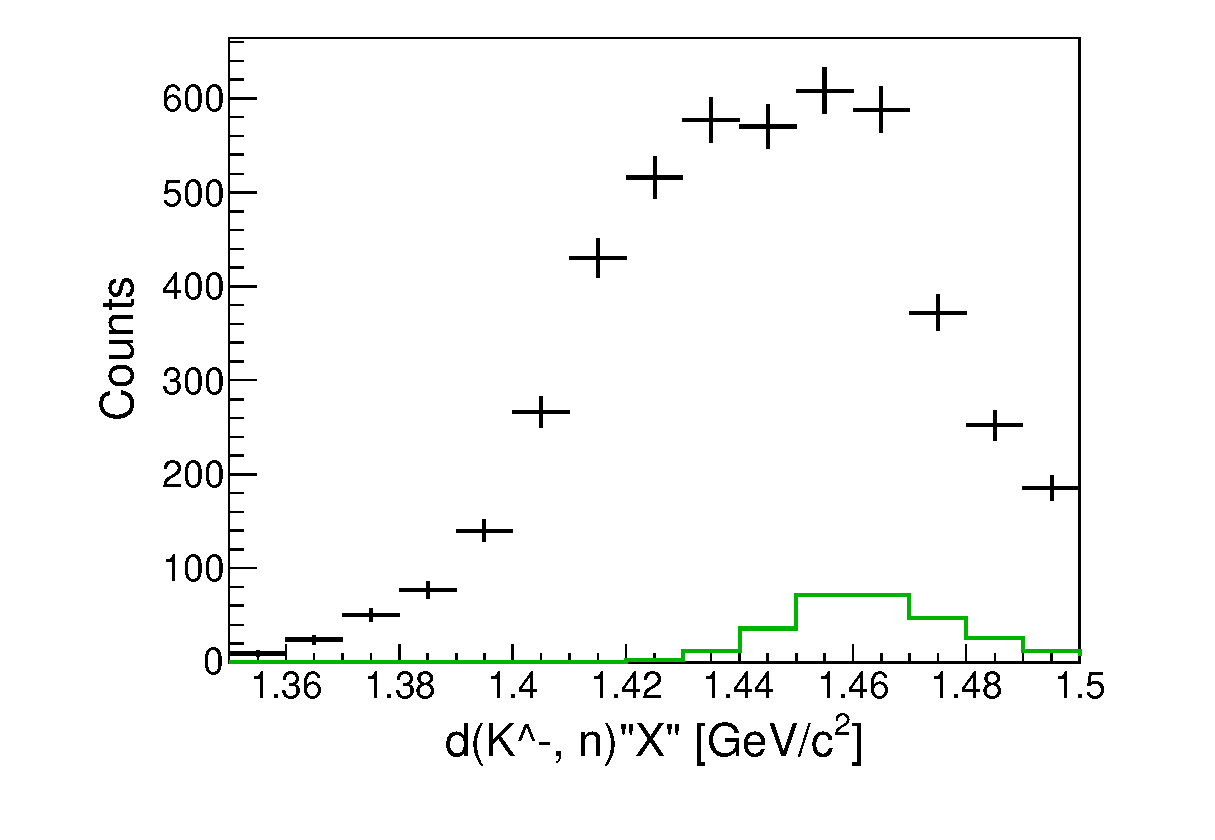
\includegraphics[width=12cm]{../pic/Run78/KN_ana_NC170_2sigma/KN_MM_woAll.eps}
  \caption{
    The figure shows $d(K^-, n)"\pi^{\pm}\Sigma^{\mp}"$ which was identified to reject events identified $K^0$ and $\Sigma_{forward}$ from detected particles.
    Color plots indicate contamination estimated by the template fitting of invariant masses.
  }
  \label{fig:KN_MM_woAll}
\end{figure}

\begin{figure}[htbp]
  \begin{tabular}{cc}
    \begin{minipage}{0.5\hsize}
      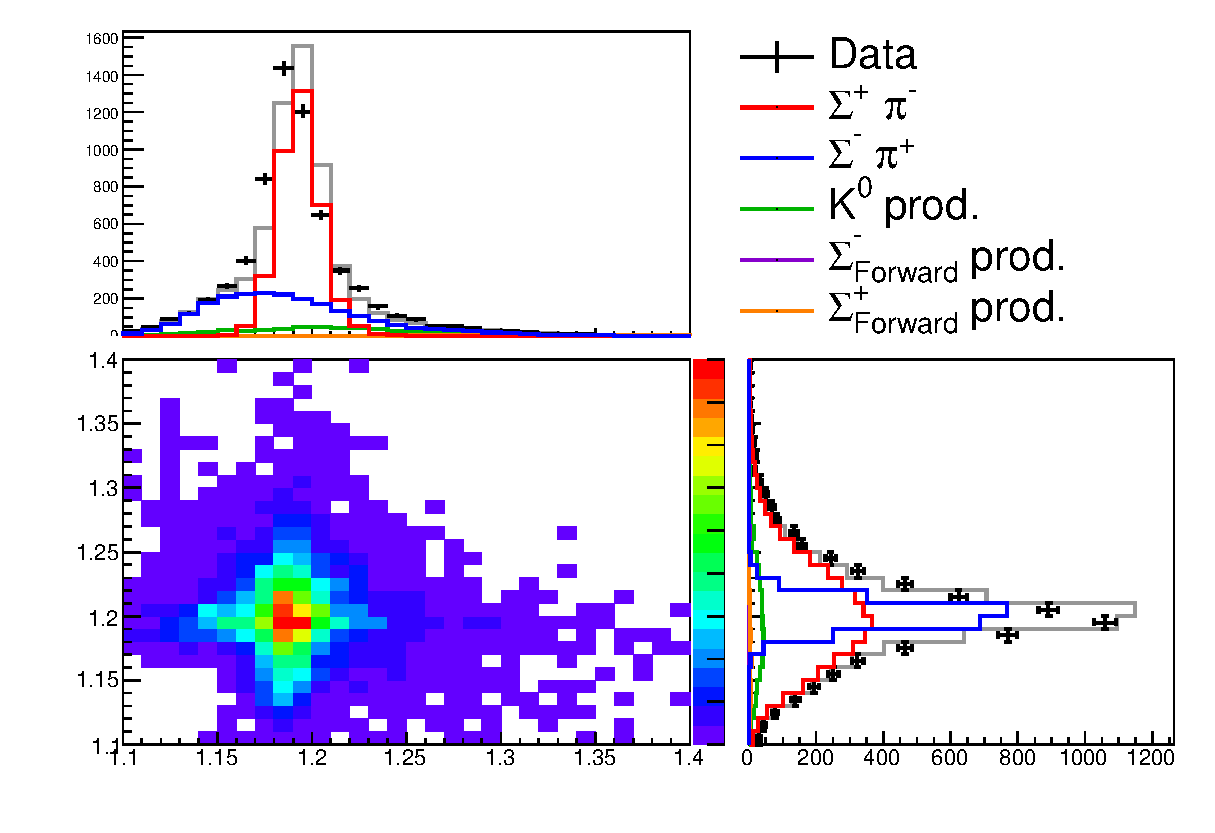
\includegraphics[width=6.5cm]{../pic/Run78/KN_ana_NC170_2sigma/KNpim_KNpip_MM.eps}
    \end{minipage}
    \begin{minipage}{0.5\hsize}
      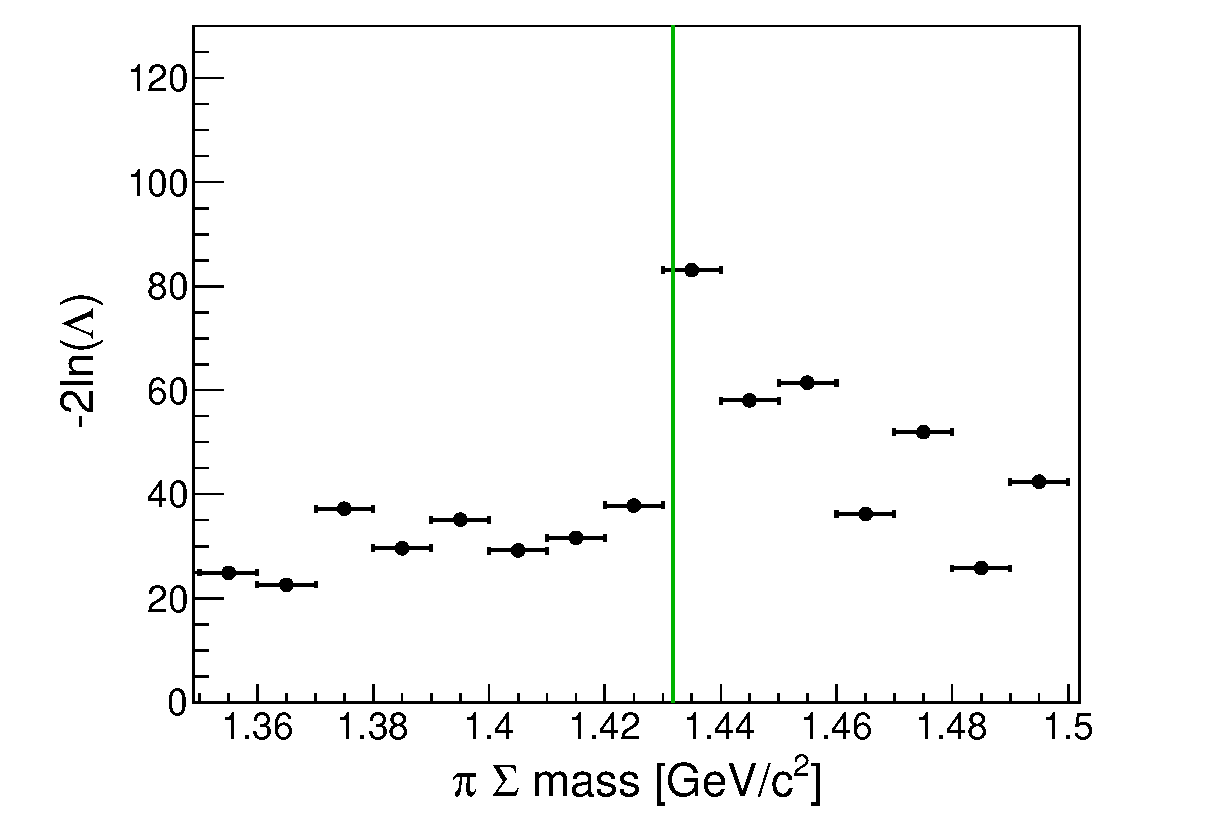
\includegraphics[width=5.5cm]{../pic/Run78/KN_ana_NC170_2sigma/Chi2.eps}
    \end{minipage}
  \end{tabular}
  \caption{
    This figure indicates summed up fitting result and log-likelihood value of each bins.
  }
  \label{fig:KNpi_MM_fit}
\end{figure}

\begin{figure}[htbp]
  \begin{tabular}{ccc}
    \begin{minipage}{0.33\hsize}
      \includegraphics[width=4cm]{../pic/Run78/KN_ana_NC170_2sigma/KNpi_MM_0.eps}
    \end{minipage}
    \begin{minipage}{0.33\hsize}
      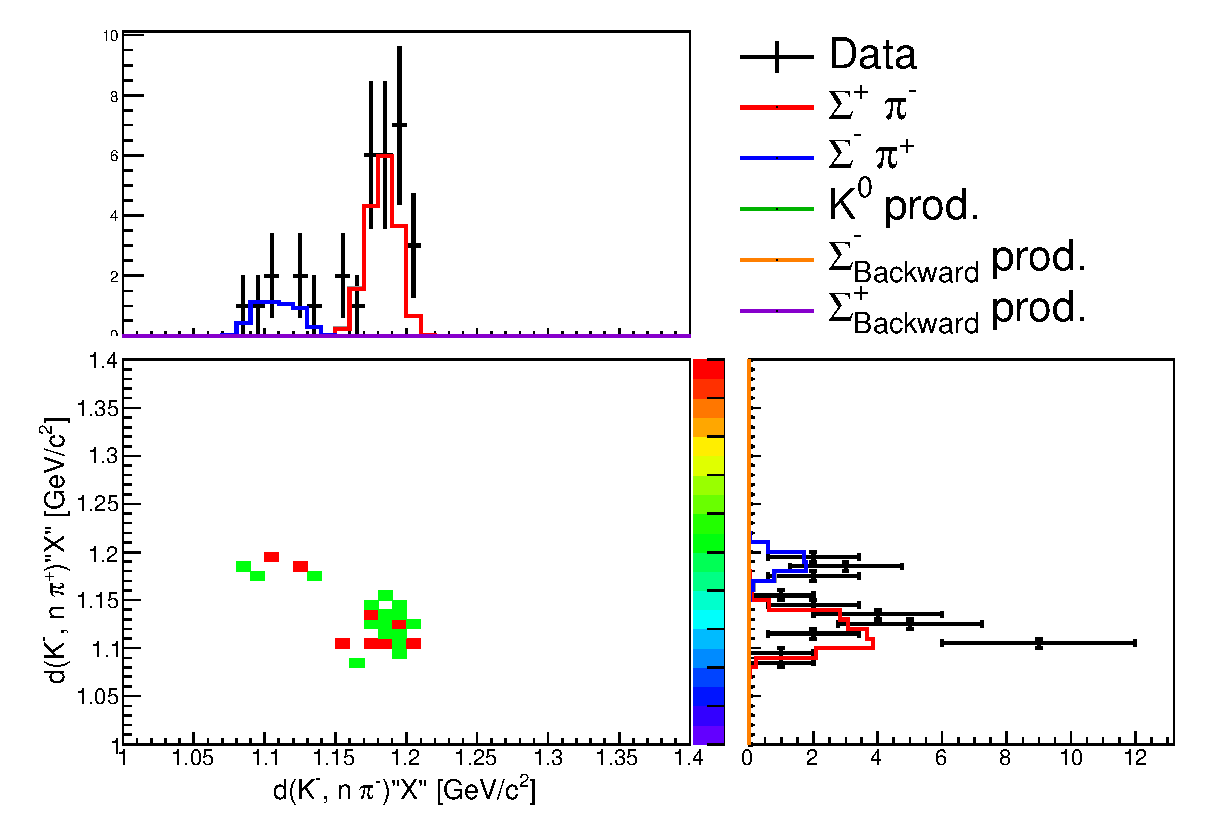
\includegraphics[width=4cm]{../pic/Run78/KN_ana_NC170_2sigma/KNpi_MM_1.eps}
    \end{minipage}
    \begin{minipage}{0.33\hsize}
      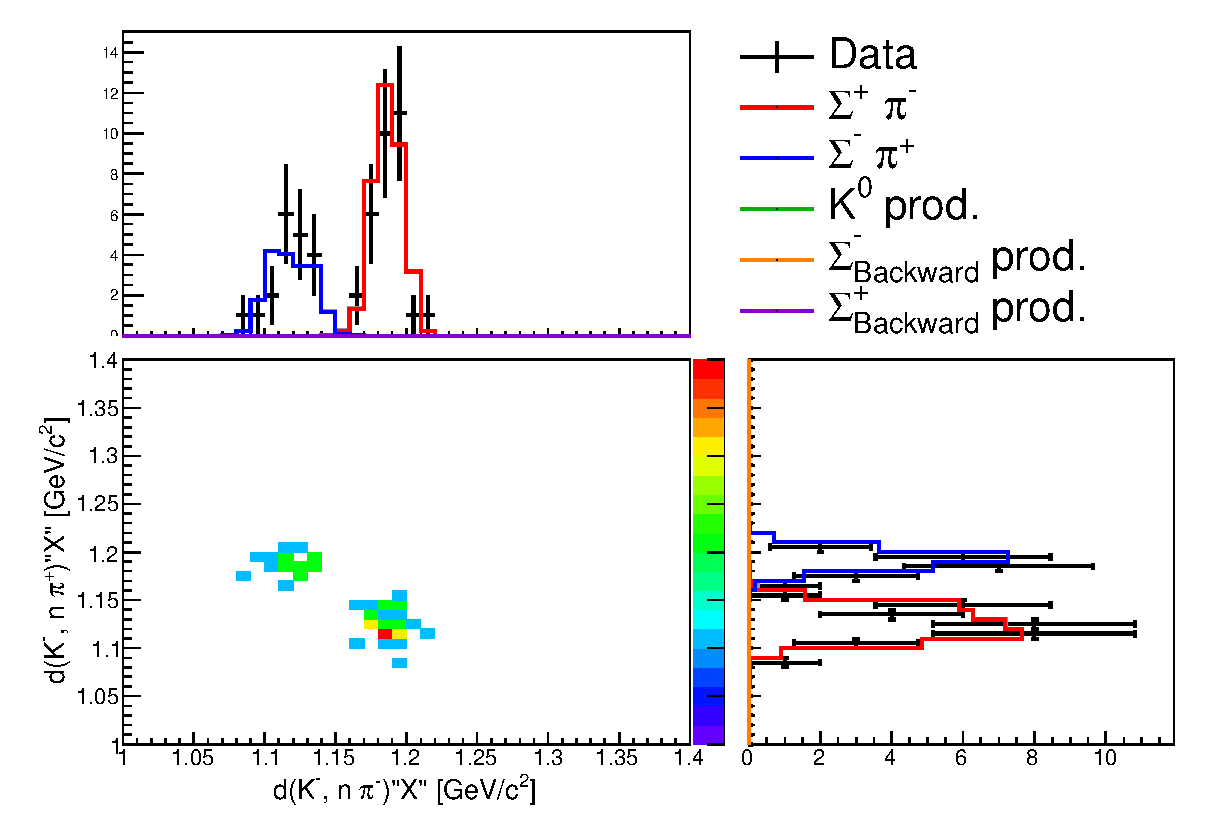
\includegraphics[width=4cm]{../pic/Run78/KN_ana_NC170_2sigma/KNpi_MM_2.eps}
    \end{minipage}
  \end{tabular}

  \begin{tabular}{ccc}
    \begin{minipage}{0.33\hsize}
      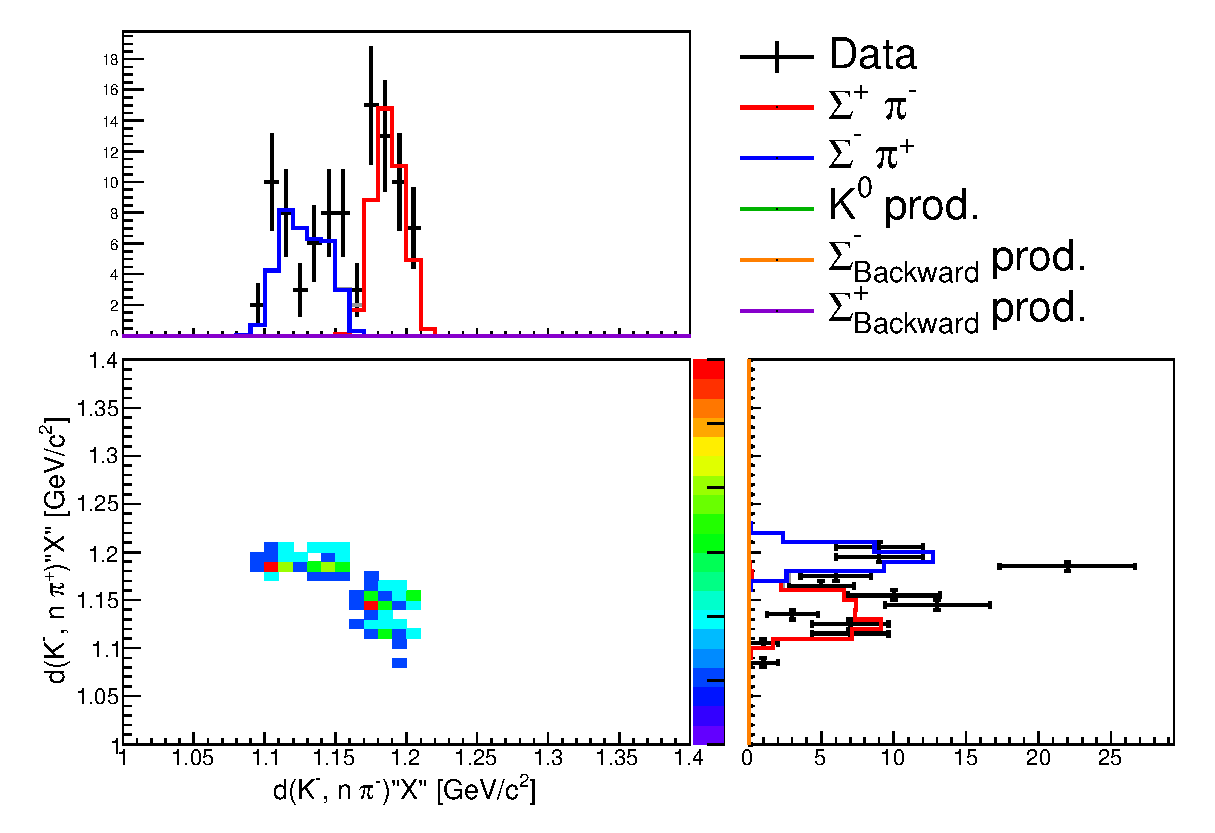
\includegraphics[width=4cm]{../pic/Run78/KN_ana_NC170_2sigma/KNpi_MM_3.eps}
    \end{minipage}
    \begin{minipage}{0.33\hsize}
      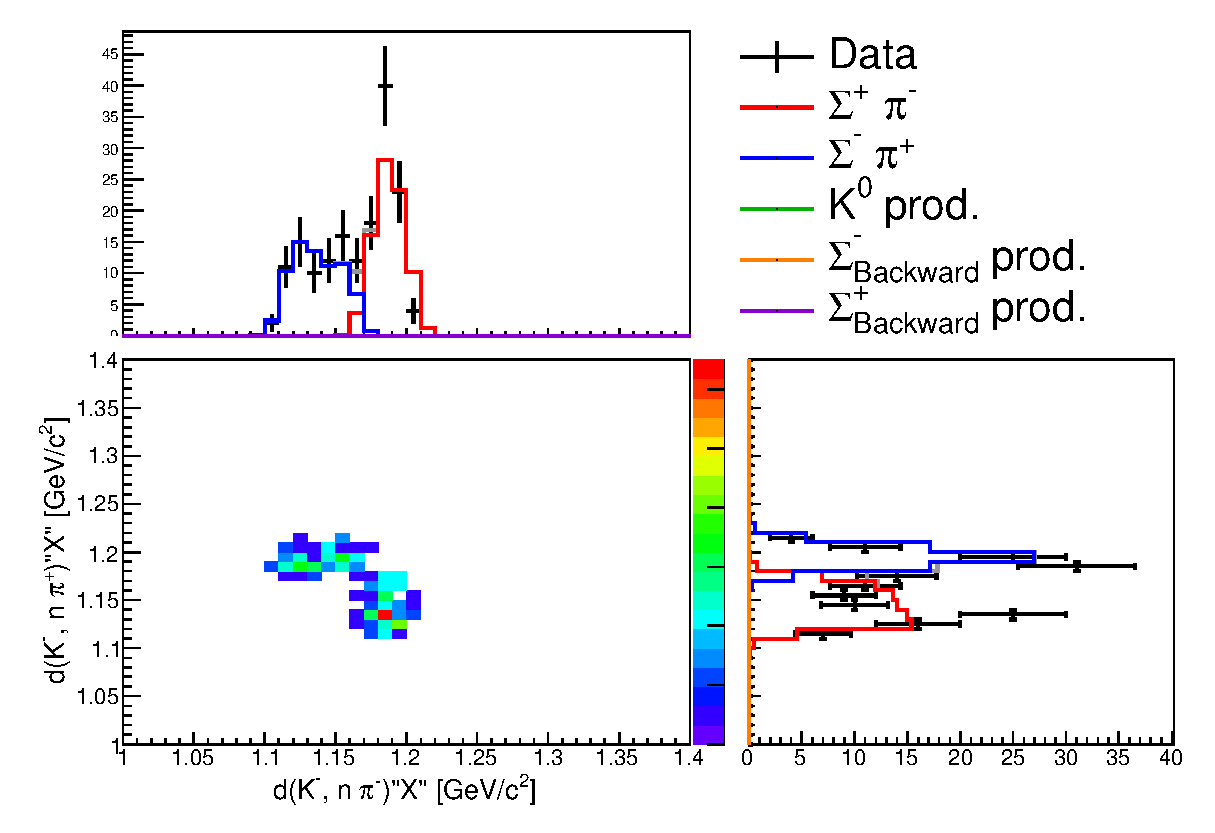
\includegraphics[width=4cm]{../pic/Run78/KN_ana_NC170_2sigma/KNpi_MM_4.eps}
    \end{minipage}
    \begin{minipage}{0.33\hsize}
      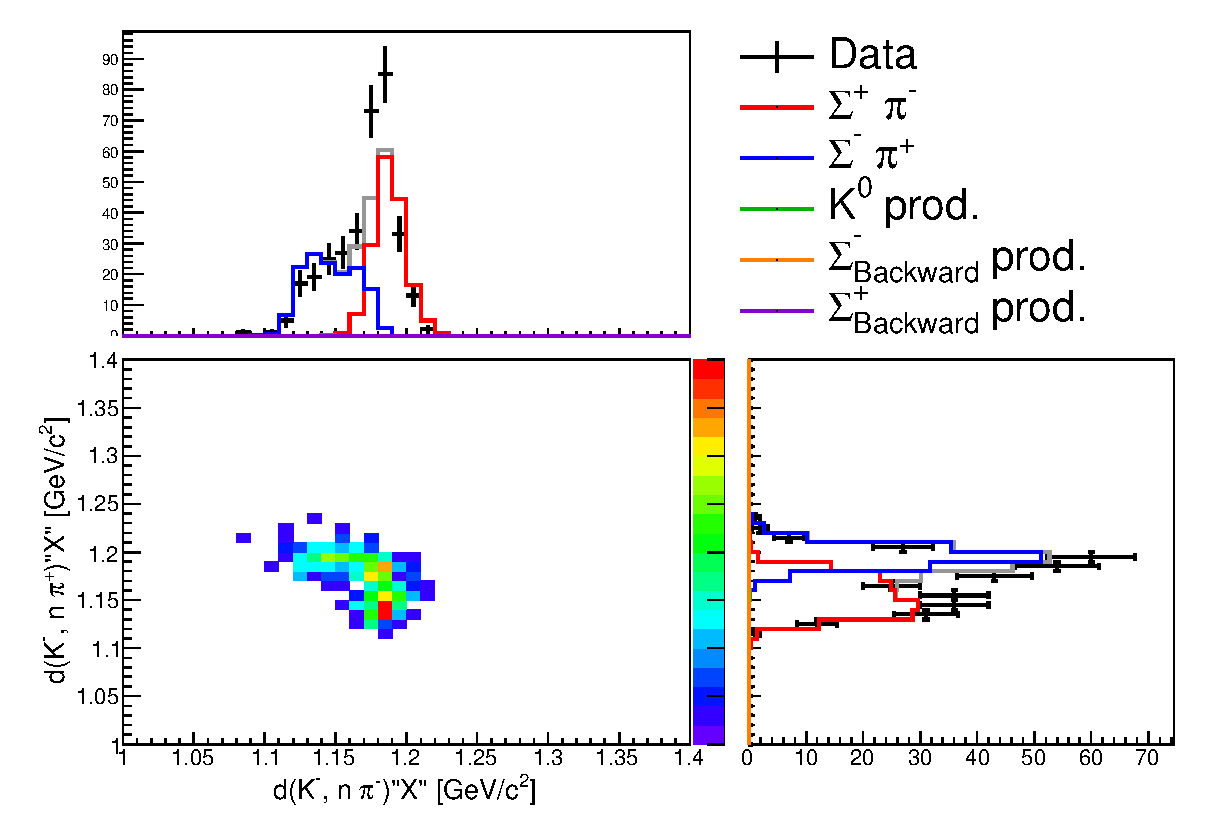
\includegraphics[width=4cm]{../pic/Run78/KN_ana_NC170_2sigma/KNpi_MM_5.eps}
    \end{minipage}    
  \end{tabular}

  \begin{tabular}{ccc}
    \begin{minipage}{0.33\hsize}
      \includegraphics[width=4cm]{../pic/Run78/KN_ana_NC170_2sigma/KNpi_MM_6.eps}
    \end{minipage}
    \begin{minipage}{0.33\hsize}
      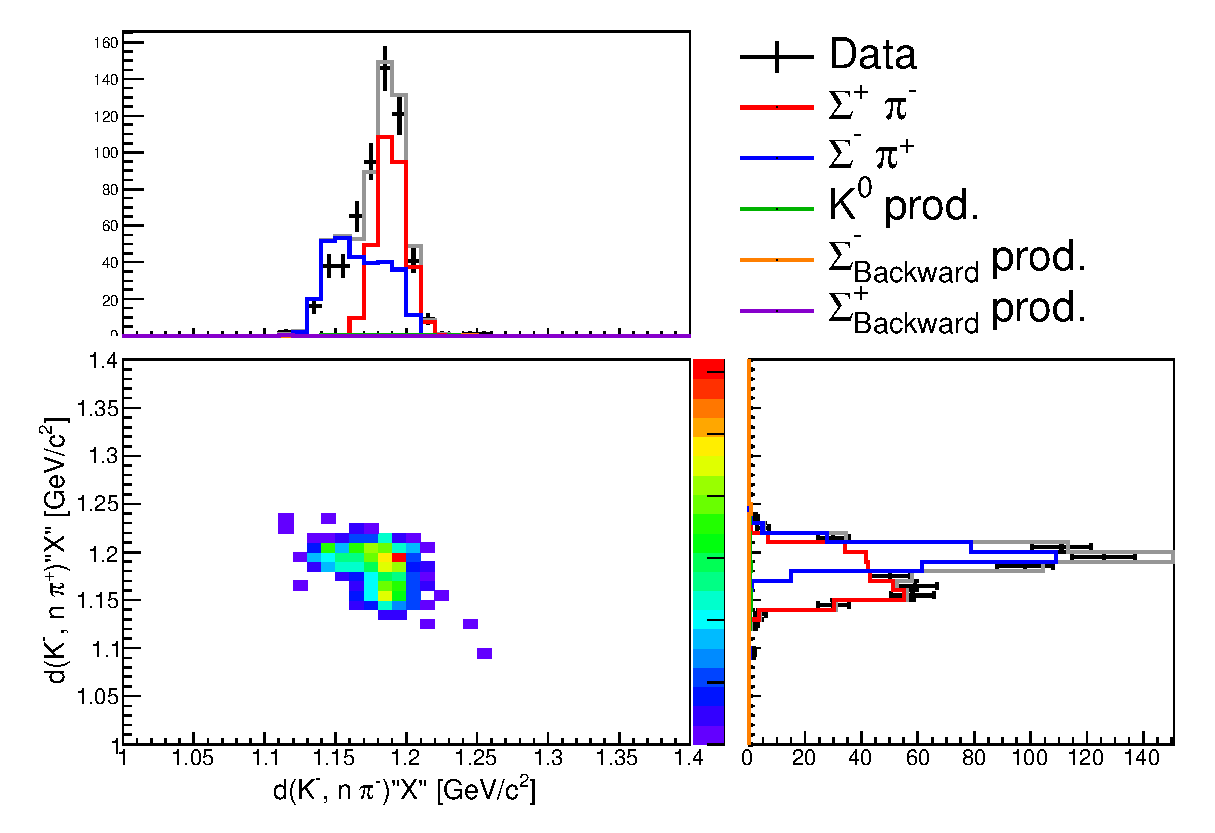
\includegraphics[width=4cm]{../pic/Run78/KN_ana_NC170_2sigma/KNpi_MM_7.eps}
    \end{minipage}
    \begin{minipage}{0.33\hsize}
      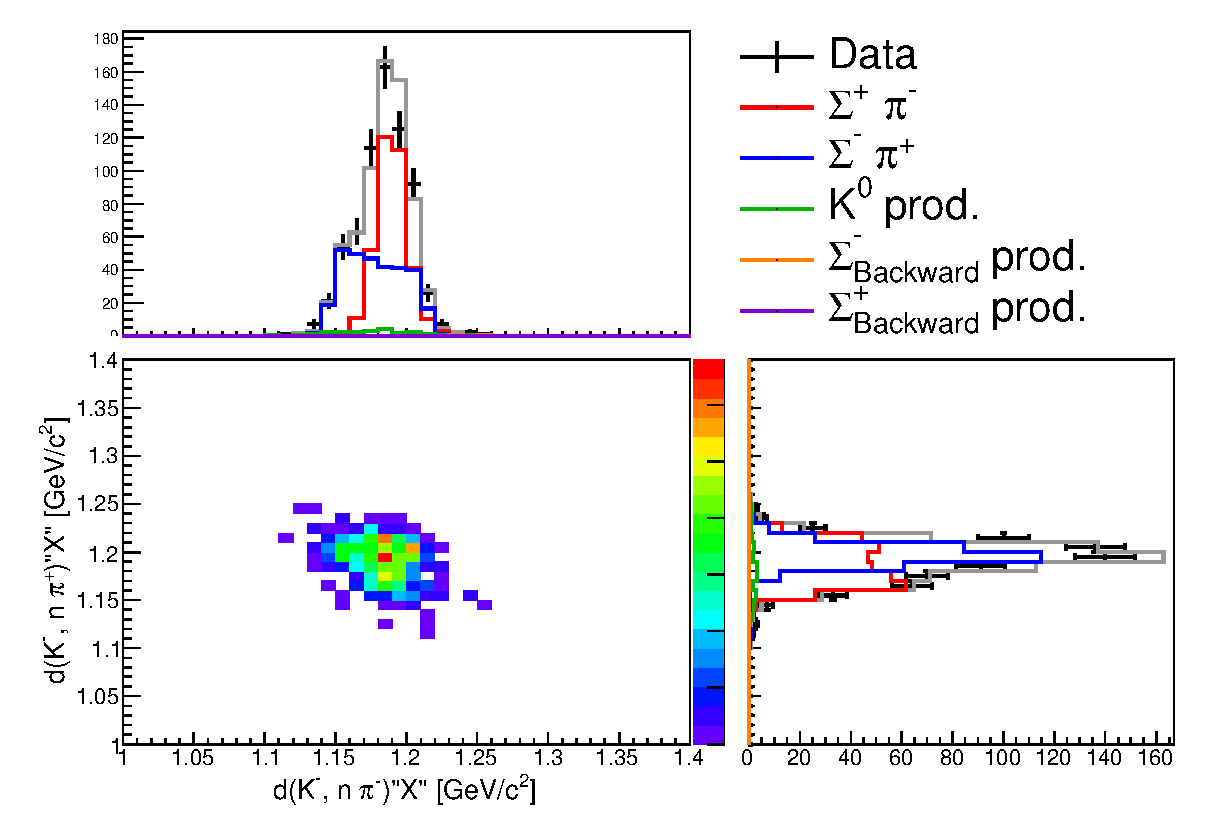
\includegraphics[width=4cm]{../pic/Run78/KN_ana_NC170_2sigma/KNpi_MM_8.eps}
    \end{minipage}    
  \end{tabular}

  \begin{tabular}{ccc}
    \begin{minipage}{0.33\hsize}
      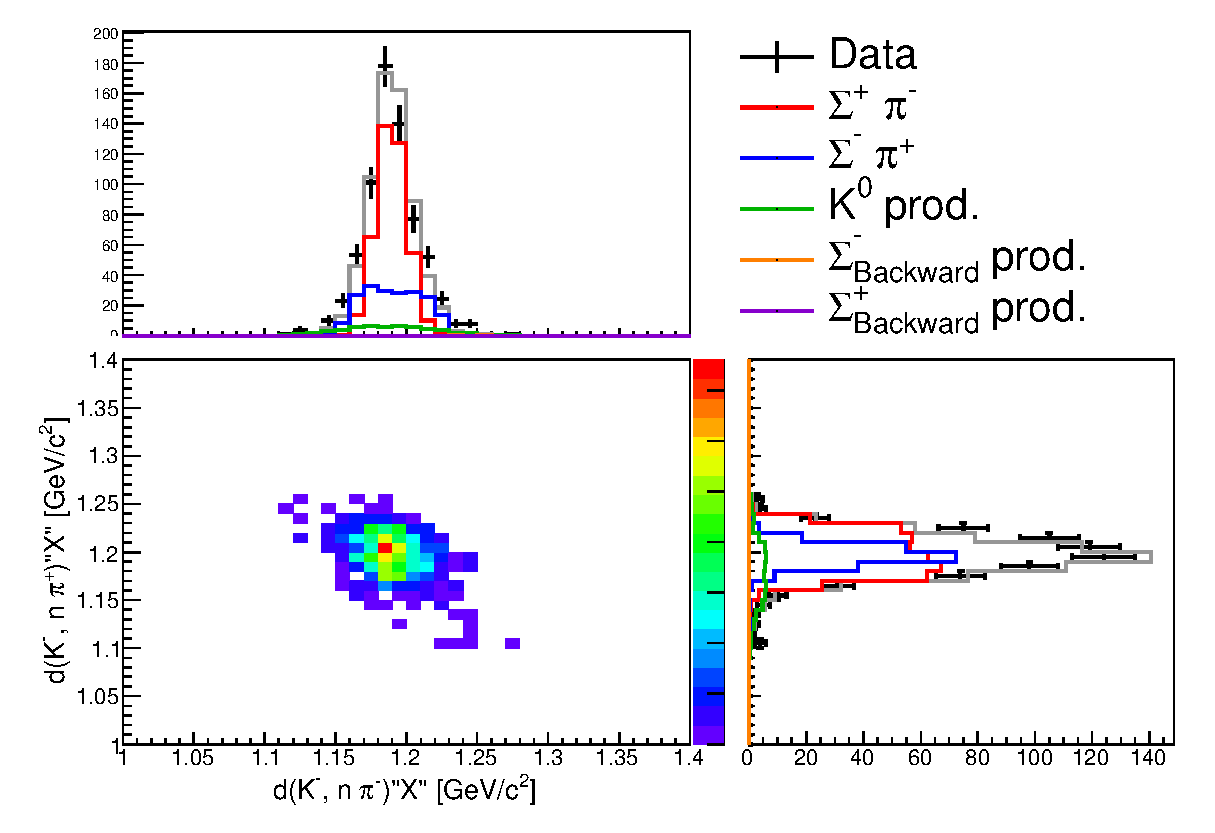
\includegraphics[width=4cm]{../pic/Run78/KN_ana_NC170_2sigma/KNpi_MM_9.eps}
    \end{minipage}
    \begin{minipage}{0.33\hsize}
      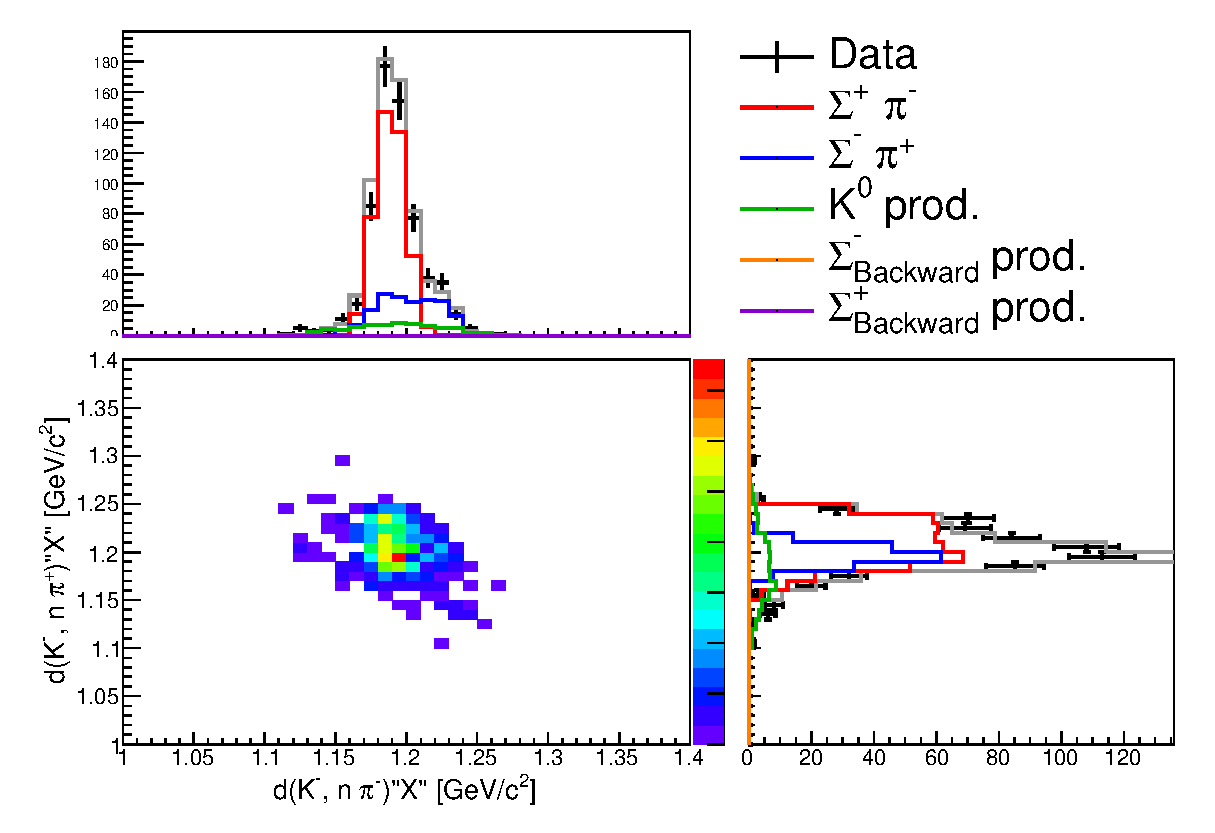
\includegraphics[width=4cm]{../pic/Run78/KN_ana_NC170_2sigma/KNpi_MM_10.eps}
    \end{minipage}
    \begin{minipage}{0.33\hsize}
      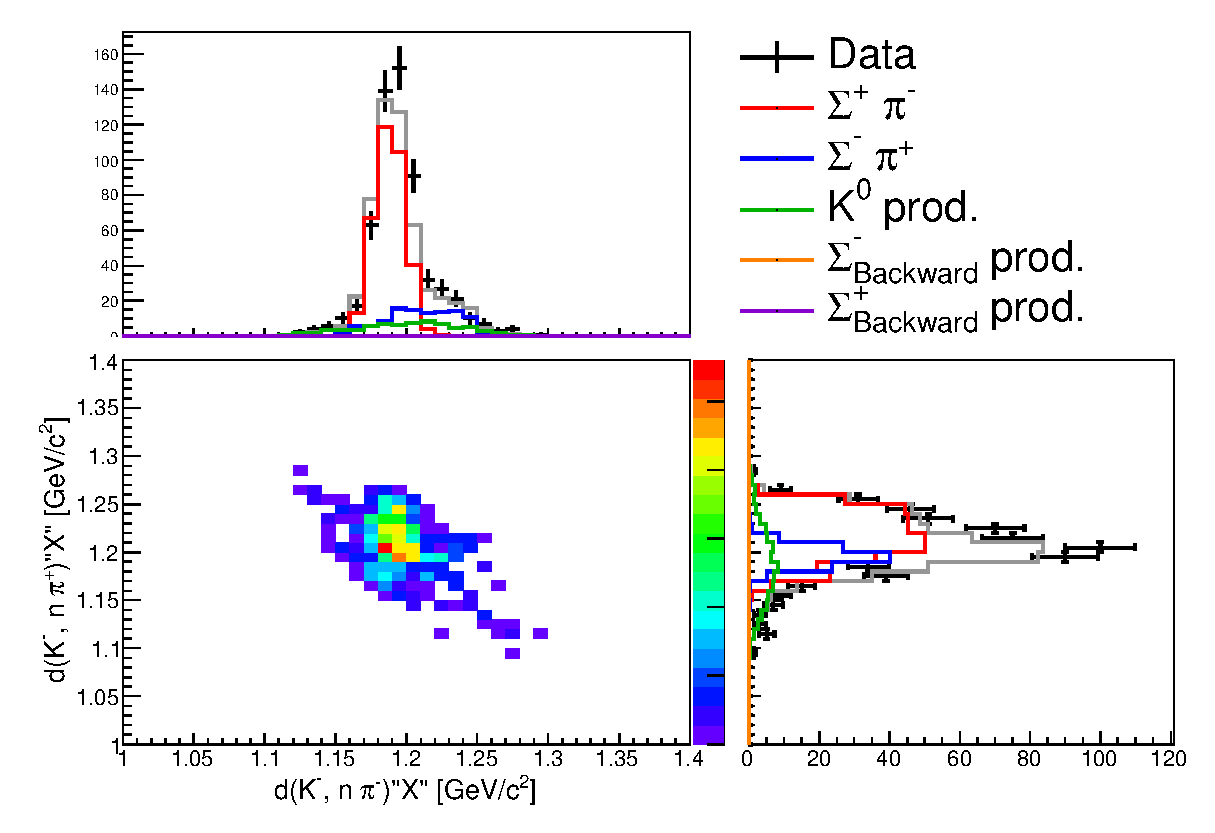
\includegraphics[width=4cm]{../pic/Run78/KN_ana_NC170_2sigma/KNpi_MM_11.eps}
    \end{minipage}    
  \end{tabular}

  \begin{tabular}{ccc}
    \begin{minipage}{0.33\hsize}
      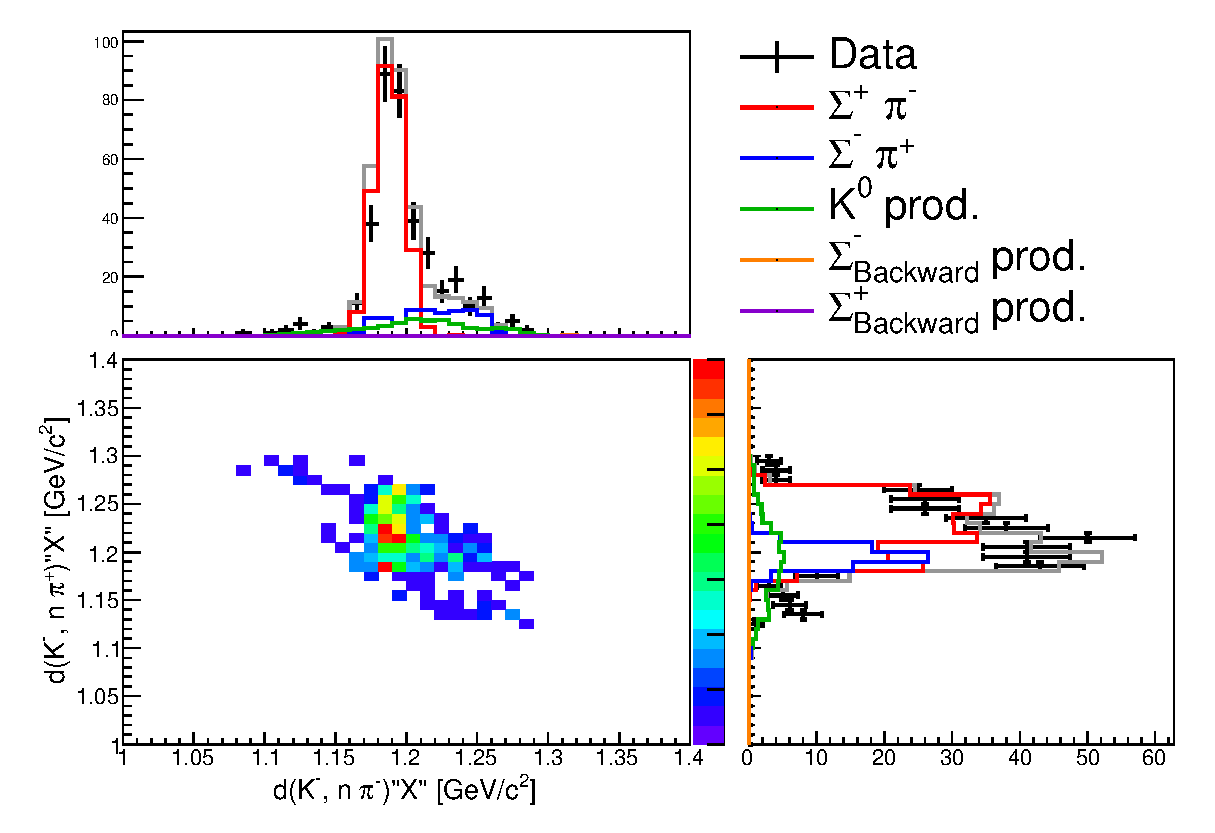
\includegraphics[width=4cm]{../pic/Run78/KN_ana_NC170_2sigma/KNpi_MM_12.eps}
    \end{minipage}
    \begin{minipage}{0.33\hsize}
      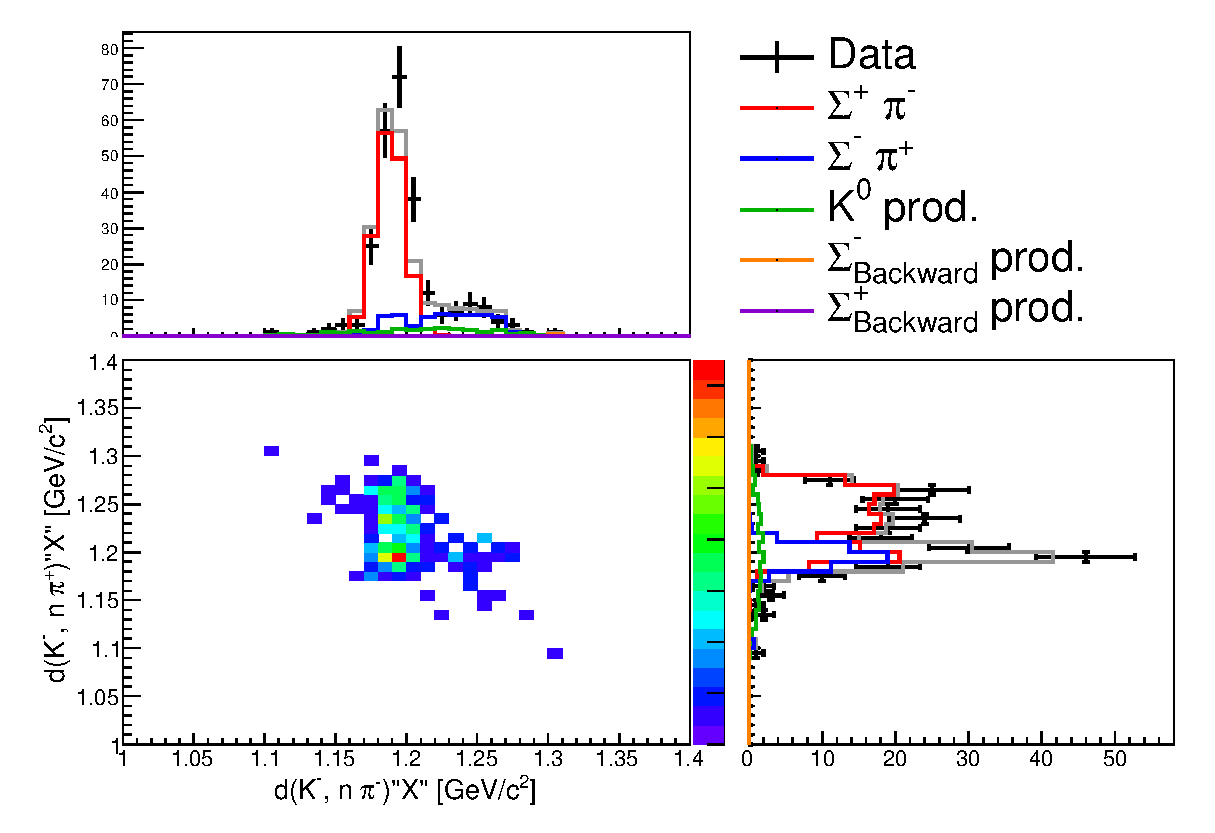
\includegraphics[width=4cm]{../pic/Run78/KN_ana_NC170_2sigma/KNpi_MM_13.eps}
    \end{minipage}
    \begin{minipage}{0.33\hsize}
      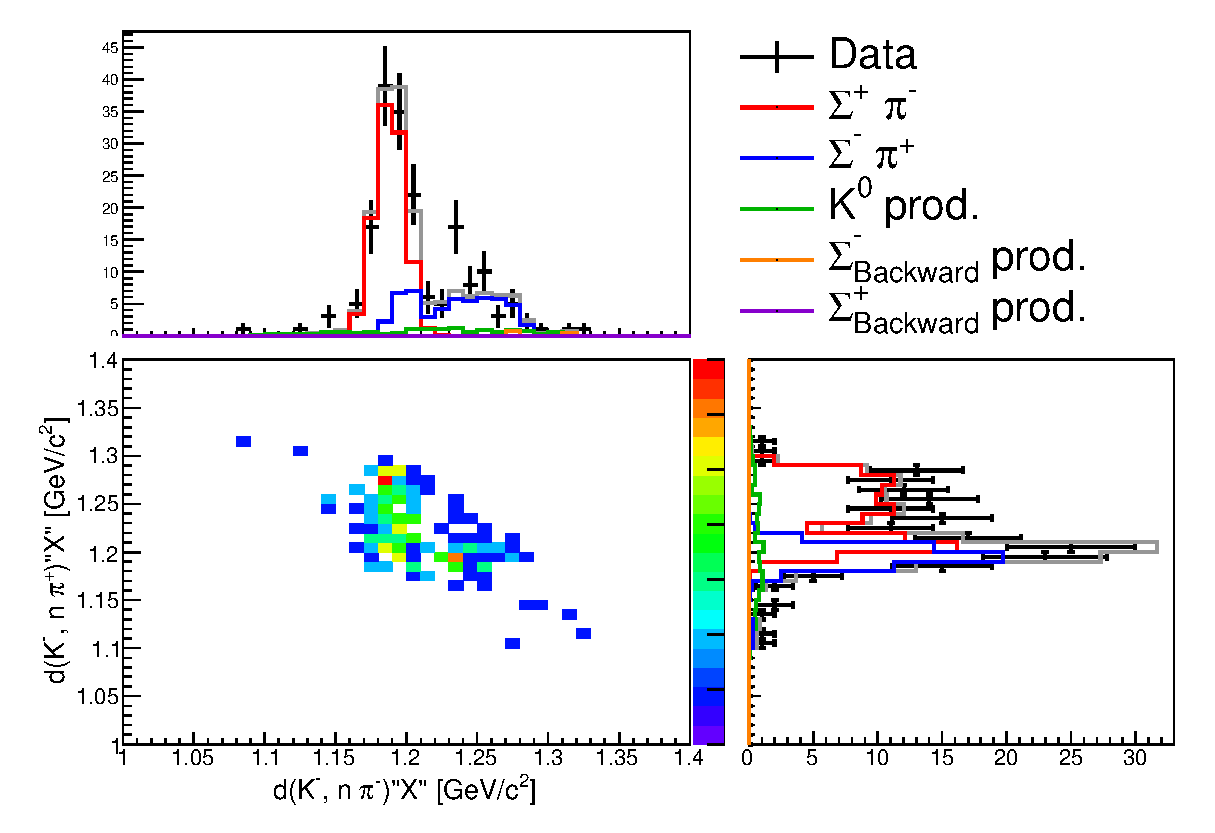
\includegraphics[width=4cm]{../pic/Run78/KN_ana_NC170_2sigma/KNpi_MM_14.eps}
    \end{minipage}    
  \end{tabular}

  \begin{tabular}{ccc}
    \begin{minipage}{0.33\hsize}
      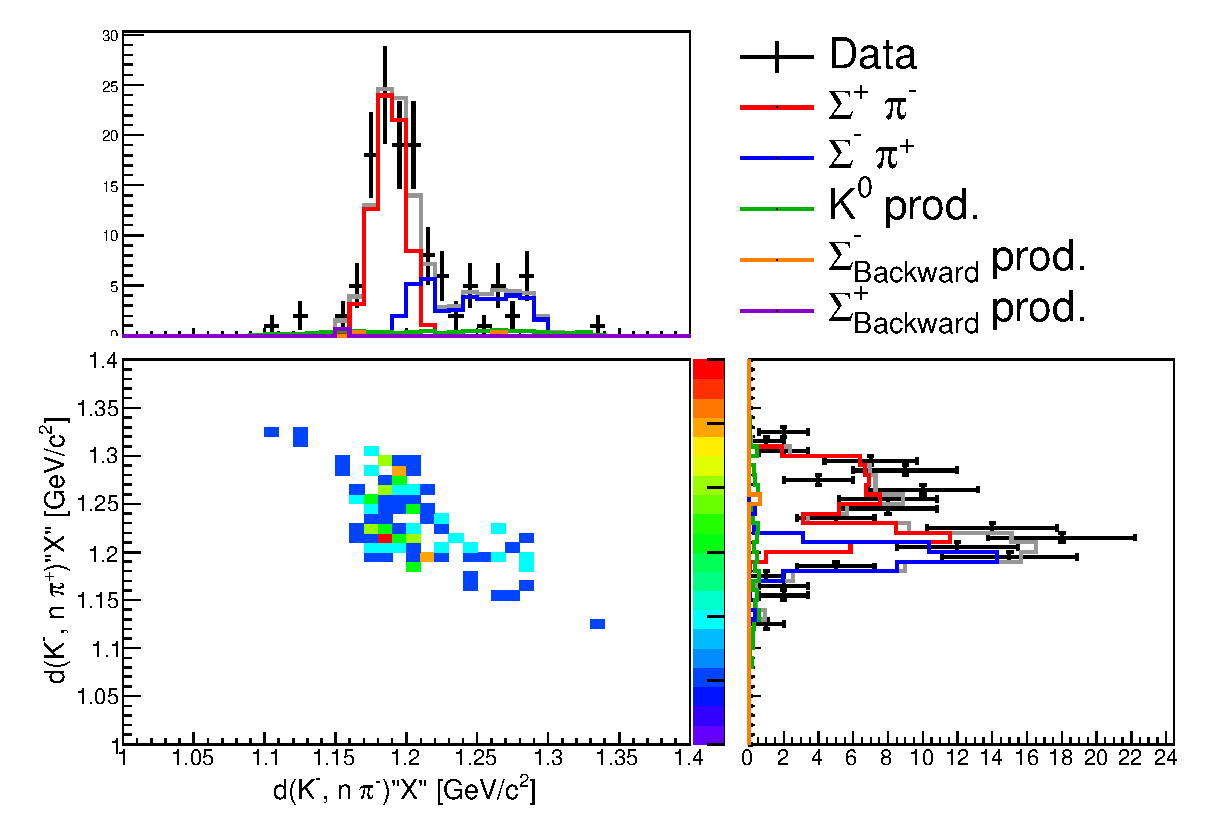
\includegraphics[width=4cm]{../pic/Run78/KN_ana_NC170_2sigma/KNpi_MM_15.eps}
    \end{minipage}
    \begin{minipage}{0.66\hsize}
      % Blank 
    \end{minipage}    
  \end{tabular}
  
  \caption{
    These figures indicate fitting results of each bins of $d(K^-, n)"\pi^{\mp}\Sigma^{\pm}"$ whose bin width is $10 MeV/c^2$.    
    Upper left figure shows about $1.35\sim1.36 GeV/c^2$ bin and the figure just to the right shows about $1.36\sim1.37 GeV/c^2$ bin.
    So, lower left figure shows about $1.49\sim1.50 GeV/c^2$ bin.
  }
  \label{fig:KNpi_MM_fit_div}
\end{figure}





\begin{figure}[htbp]
  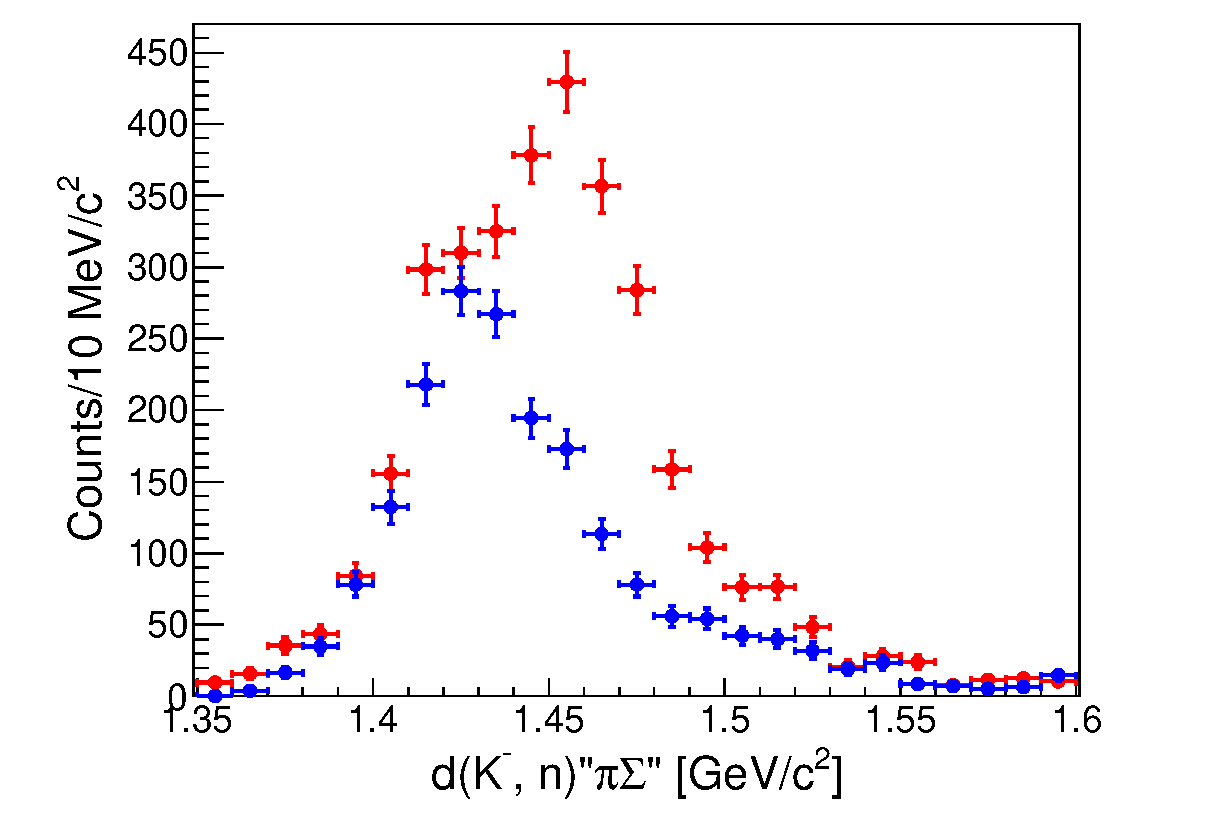
\includegraphics[width=12cm]{../pic/Run78/K0_ts_L1520/before_after.eps}
  \caption{
    This figure indicates decomposed number of $d(K^-, n)"\pi^-\Sigma^+"$ and $d(K^-, n)"\pi^+\Sigma^-"$ modes.
    In this figure, $K^0$ 2-step reaction effect is including which discribed Sec.\ref{sec:K0_2step}.
  }
  \label{fig:ChargeNum}
\end{figure}


